\documentclass[10pt,twocolumn,letterpaper]{article}

\usepackage{cvpr}
\usepackage{times}
\usepackage{epsfig}
\usepackage{graphicx}
\usepackage{amsmath}
\usepackage{amssymb}

% Include other packages here, before hyperref.

% If you comment hyperref and then uncomment it, you should delete
% egpaper.aux before re-running latex.  (Or just hit 'q' on the first latex
% run, let it finish, and you should be clear).
\usepackage[breaklinks=true,bookmarks=false]{hyperref}

\cvprfinalcopy % *** Uncomment this line for the final submission

\def\cvprPaperID{****} % *** Enter the CVPR Paper ID here
\def\httilde{\mbox{\tt\raisebox{-.5ex}{\symbol{126}}}}

% Pages are numbered in submission mode, and unnumbered in camera-ready
%\ifcvprfinal\pagestyle{empty}\fi
\setcounter{page}{1}
\begin{document}

%%%%%%%%% TITLE
\title{Artificial Intellegence Project Report: Route Planning}

\author{Author\\
Yifei Chen, Yao Gu, Qichen Gao, Shuai Yan, Changming Li}

% For a paper whose authors are all at the same institution,
% omit the following lines up until the closing ``}''.
% Additional authors and addresses can be added with ``\and'',
% just like the second author.
% To save space, use either the email address or home page, not both

\maketitle
%\thispagestyle{empty}

%%%%%%%%% ABSTRACT
\begin{abstract}
   Since path planning questions have many mutations, different method can be applied to pan the route in different situations. 
   We have made some modifications on the basis of the mathematical modeling competition topics in 2020b, 
   obtained the path planning scenarios in this paper, and hope to find the optimal path to meet the requirements 
   of the problem through MDP. 
   We try to analysis the advantages and disadvantages of MDP in this situation.

\end{abstract}

%%%%%%%%% BODY TEXT
\section{Introduction}

Motion planning is composed of path planning and trajectory planning,
 the sequence points or curves connecting the starting and ending 
 positions are called paths, and the strategies that make up the 
 path are called path planning. We choose one of the path planning 
 situation to apply our method.

%-------------------------------------------------------------------------
\subsection{Route Planning Question}

Given a map consist of several regions, with one start point and 
one goal point. Player need to cross the dessert to the goal point 
with as much resources as possible. Before heading into the desert, 
you have some initial resources. For each state, its value will be shown 
on the screen. There are two choices for every day to choose: go in one 
direction and stay. In the desert, you need to consume a certain amount 
of supplies every day. Once the supplies are used up, or after 30 days 
you do not reach the goal, the game fails. There are different 
weathers on each day: "high temperature" leads to a higher consumption 
of supplies; "sandstorm" forces you to stay in one place for that 
day; "sunny" days just normal. There is also a mine in the desert, 
where you can mine and get money from it (you cannot move that day of course)


\subsection{Route Planning With Precise Weather Or Random Weather}

In the first scene, we know every day's weather for sure. With this ability, we should
figure out an optimal path for the question.while in the second one we only know about the probability of each day's weather.
So for this part, we should design a best path considering the uncertain weather.

\section{Mathematics}
Markov decision process (MDP) provides a mathematical framework for modeling decision 
making in situations where outcomes are partly random and partly under the control of 
an agent. It is a discrete time stochastic control process, where agents must make 
decisions under uncertainty by comparing the values of actions that gather information 
and immediate reward. 
\\MDPs are widely used in many fields, such as robotics, automatic control, economics, 
and manufacturing. The name of MDPs comes from the Russian mathematician Andrey Markov 
as they are an extension of Markov chains. 'Markov' generally means that given the 
present state, the future and the past are independent. 
For Markov decision processes, ��Markov�� means action outcomes depend 
only on the current state. This is just like search, where the successor 
function could only depend on the current state (not the history).

\subsection{MDP method}
An MDP is defined by: a set of states $s \in S$, a set of actions $a \in A$,
a transition function $T(s, a, s')$ which serves as the probability that action $a$ 
from state s leads to state $s$, a reward function $R(s, a, s')$, a start state 
and maybe a terminal state. For MDPs, we usually want an optimal policy $\pi^* $ 
which is mapping form states to actions, in other words, we want to extract a list 
of optimal actions from the states. For optimal we mean maximizing expected utility 
for example sum of rewards. MDPs are non-deterministic search problems which can be 
solved by expectmax search. However, using expectmax search will suffer from multiple 
repeated states for search and the problem of unlimited depth. Thus, a new 
method is introduced called value iteration. For value iteration, we need 
to introduce several quantities. The first one is value $V(s)$ which is defined as 
expected utilities starting in state $s$ and the other one is $\pi (s)$ which is the action from state $s $
also called policy. 

\subsection{MDP Path Planning}
In value iteration $V_k(s)$ is defined as the optimal value of state $s$ if the game ends in$ k $more time 
steps.The main steps of value iteration are shown below. We start with $V_0(s) = 0$ because we expected zero 
reward when no time steps left. For exit state, we give it a reward with $R(s,a,exit\_s) = 2000$ to make it tend to exit.
For those unliked terminal state $s'$ for instance, out of date, we give it a penalty with $R(s,a,s') = -200000$ to
make it avoid entering these state.

Then given vector of  $V_k(s)$ values, do one ply of expectimax from each state using 
the formula: $$V_{k+1}(s) = \max_a{\sum_{s'} T(s,a,s')[R(s,a,s')+\gamma V_k(s')] } $$

We repeat it until convergence. Finally, we need to extract the policy by:
$$\pi^* (s) = argmax_{a}\sum_{s'}T(s,a,s')[R(s,a,s')+\gamma V_k(s')]$$

But it is easier using Q value than value, therefore we compute Q values:
$$Q(s) = \sum_{s'}T(s,a,s')[R(s,a,s')+\gamma V_k(s')]$$
Thus, we compute the Q value instead.

\section{Path Planning Code Design}
\subsection{Code}
In mdp.py, we implemented the core function and components of MDP 
including obtaining successors, the states, actions, transition 
function and rewards etc. For successors, we must first check their 
validity then check whether they are terminals. We have to encode different 
information for specific states such as mining and village. We set different 
rewards and consumption according to different situations including weathers 
and terminations. For extracting actions, we first get the neighbors of the 
current states and return actions based on whether it is a normal state. 
In valueIterationAgents.py, the discount factor and number of iterations 
are set by default with 0.9 and 100 respectively. In order to get a path 
for visualization we iterate to find the list of states with maximum value 
and after that we are able to find out the value along the path. For policy 
extraction, we make use of the Q values computed from values in 
��computeQValueFromValues�� function. In graph.py, we have the 
2 graphs for the problem which is manually typed in and a random weather 
generator is also included.

\subsection{Graph User Interface}
In order to make user easier to view our figured path, we design a GUI for our code.
In ui.py, we visualized the process of the player crossing the map. 
The point represents the state: yellow means mining and green means walking. 
The black circle shows the start or goal point. 
The lines represent the route of the player and they will change color if 
they were passed again. Finally, the UI shows the days remain and the v-value 
at the botto-left corner as you can see in Figure 1.

What's more we also allow user to change the location of the start, end, even the mine. 
For more detailed information about how to run the code, please refer to the readme.md file
in the code zip.
\begin{figure}[t]
   \begin{center}   
   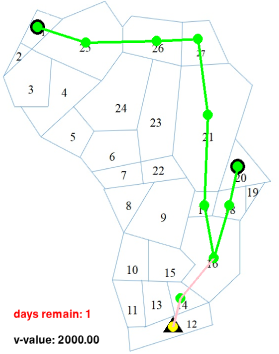
\includegraphics[width=0.8\linewidth]{sample.png}
   \end{center}
      \caption{Example of the graph user interface. 
      The start point and the end point are circled out. 
      And for the mine, it is labeled by a traingle. 
      For the yellow circle, 
      it means that we are mining at this position}
   \label{fig:long}
   \label{fig:onecol}
   \end{figure}


\subsection{Advantages \& Disadvantages}
Disadvantages: Since we are using value iteration, the time complexity 
is $O(S^2 A)$ which is quadratic to the number of states and linear to 
number of actions makes our algorithm a bit slow. 
We apply it because it is ensured to have an optimal solution. 
Besides if the state space is too large and the state is too complex, 
we need more time to find an answer. 
Therefore, we simplify the design of states as mentioned by Professor Tu.

Advantages: An MDP is quite suitable for our topic which is making 
decisions in an uncertain environment. It turns out to be that MDP 
usually achieve good performance in our problem. It is convenient to 
make changes to different conditions such as revising the transition 
function for weather and the rewards to test for our implementation.

\section{Conclusion}
For this kind of path planning problem that may occur in reality, 
we can solve this problem by applying MDP properly. Although the time 
complexity may be high due to the large number of states and actions, 
it can always find an optimal solution. For further study, a supplemental 
station may be added to the game to make the game more realistic.


%-------------------------------------------------------------------------
\section{References}

Our project do not refer much code from others. Only a data structure file from UC Berkley.
Besides, our inspiration comes from Mathematical Modeling Competition 2020b.
\begin{center}
   1. Mathematical Modeling Competition 2020b
\end{center}

\end{document}
